\documentclass[journal=jpccck,manuscript=article]{achemso}

\usepackage{hyperref}

\usepackage{siunitx}
\DeclareSIUnit\rydberg{Ry}
\usepackage{tikz}
\usepackage{paralist}
\usepackage[version=4]{mhchem}
\usepackage{booktabs}
\usepackage{rotating}
\usepackage{chngcntr}


\author{Pierre Beaujean}
\affiliation[Unamur]
{University of Namur, Theoretical Chemistry Lab, Unit of Theoretical and Structural Physical Chemistry, Namur Institute of Structured Matter, rue de Bruxelles, 61, B-5000 Namur (Belgium)}


\author{Benoît Champagne}
\affiliation[Unamur]
{University of Namur, Theoretical Chemistry Lab, Unit of Theoretical and Structural Physical Chemistry, Namur Institute of Structured Matter, rue de Bruxelles, 61, B-5000 Namur (Belgium)}
\email{benoit.champagne@unamur.be}

\title{Prediction of XPS binding energies for molecules grafted on calcium surfaces\\Supporting information}

\def\dbe{\ensuremath{\Delta\text{BE}}}



\renewcommand{\thetable}{S\arabic{table}}
\renewcommand{\thefigure}{S\arabic{figure}}

\begin{document}
	\maketitle

\begin{figure}[!h]
	\centering
	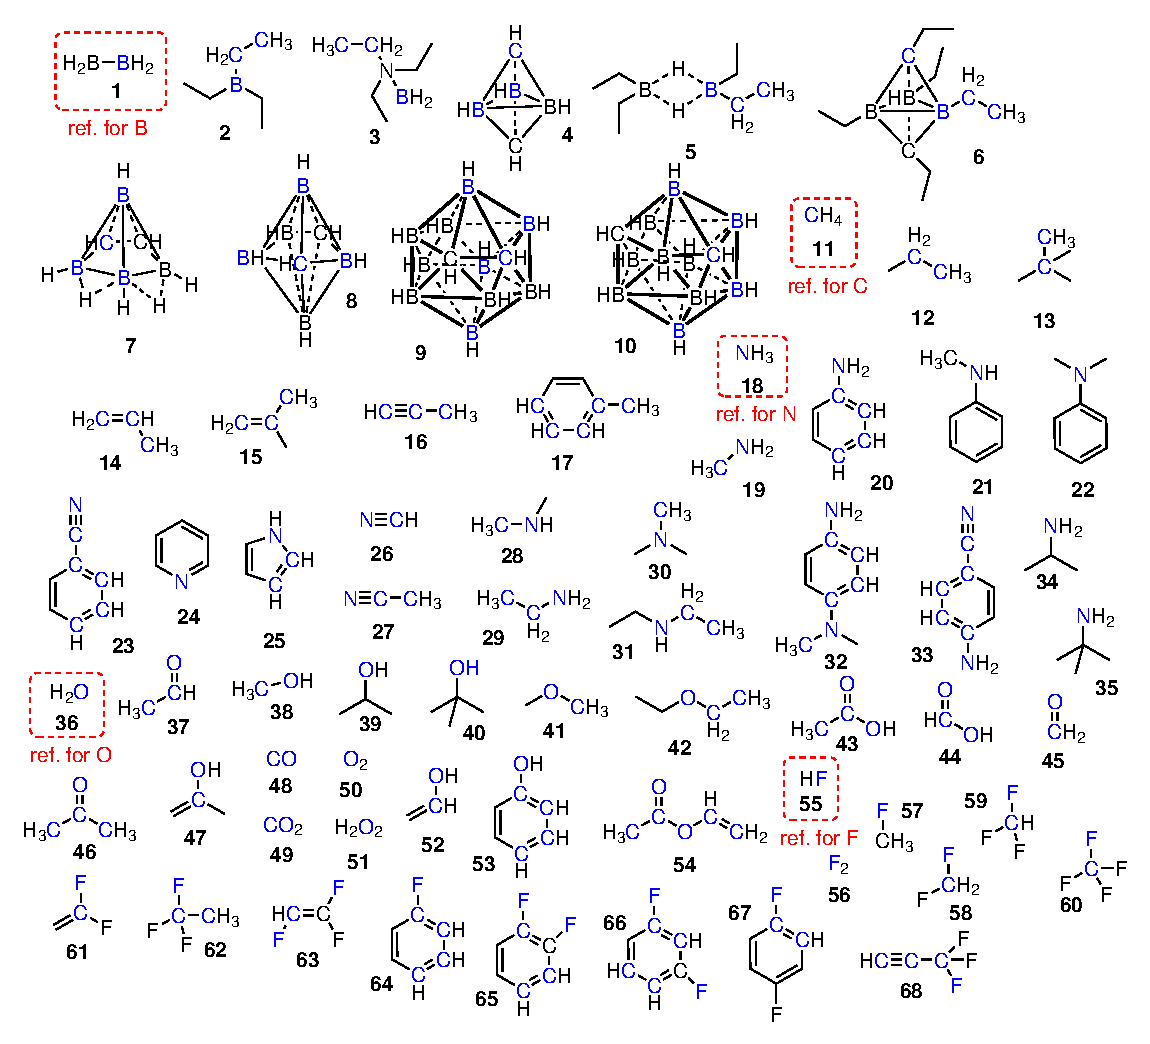
\includegraphics[width=\linewidth]{FigureS1}
	\caption{Molecules for the benchmark , from Ref.~\citenum{pueyobellafontPredictingCoreLevel2017}. The atoms for which experimental BE are provided are highlighted in blue.  The reference compounds used for each atom are highlighted in red.}
	\label{fig:core185}
\end{figure}


\begin{figure}[!h]
	\includegraphics[width=\linewidth]{FigureS2}
	\caption{Evolution of the surface energy for slabs of Ca, CaO, and \ce{CaH2} with increasing thickness ($N$) , as estimated by least-square fit of Eq.~(5). For CaO, the surface energies of (110) and (111) are larger than \SI{1.25}{\joule\per\meter\squared}.}
	\label{fig:surf}
\end{figure}

\begin{table}[!h]
	\begin{tabular}{c ccc c ccc cl}
		\toprule
		Ca & & \multicolumn{2}{c}{CaO} & & \multicolumn{3}{c}{\ce{CaCO3}} & Ref. & Note\\
		\cline{1-1} \cline{3-4} \cline{6-8}
		Ca 2s & & Ca 2s & O 1s  & & Ca 2s & O 1s & C 1s\\
		\midrule
		438.8 & &---&---&& --- & --- &--- & \citenum{fuggleCorelevelBindingEnergies1980} & Relative to VBM\\
		436.6 & & 437.9 & 528.9& & 439.1 &531.6 & 289.7& \citenum{sosulnikovXrayPhotoelectronStudies1992}& Relative to C 1s = \SI{285.0}{\electronvolt}\\
		 --- && 437.4 & 531.2&& 437.8 & 531.0 & 289.0 & \citenum{demriXPSStudyCalcium1995} & Relative to C 1s = \SI{284.6}{\electronvolt}\\
		 $\sim$450 & & 441.0 & 532.2 & & --- & --- & --- & \citenum{ochsCO2ChemisorptionCa1998} & Relative to $E_F$ \\
		 --- & & 439.0 & 531.9 & & 438.4 & 531.4 & 285.4 & \citenum{cristHandbookMonochromaticXPS2000a} & Relative to C 1s = \SI{285.0}{\electronvolt}\\
		 442.5 & & 438.15 & 531.15 & & 439.08 & 531.58 & 290.08 & \citenum{cristXPSLibraryWebsite2021a} & Relative to C 1s = \SI{285.0}{\electronvolt}\\
		\bottomrule
	\end{tabular}
	\caption{Value of peak maximum energies for Ca, CaO, and  \ce{CaCO3}, from different sources. It is now recognized than for surfaces, a peak is not necessarily equivalent to a single binding energies (peak fitting is required), and that the spectra for pure CaO are difficult to obtain without contamination.}
\end{table}

\newcommand{\XPSsa}[3]{
	\begin{figure}[!h]
		\centering
		\includegraphics[width=.8\linewidth]{Figure#1a}
		\includegraphics[width=.8\linewidth]{Figure#1b}
		\caption{Difference (dotted line) between the XPS spectrum before (dashed line) and after (plain line) adsorption for compounds \textbf{#2} (top) and \textbf{#3} (bottom) on the different substrates.}
		\label{fig:spectraXPSads#2#3}
	\end{figure}
}

\XPSsa{S4}{a}{b}
\XPSsa{S5}{c}{d}
\XPSsa{S6}{e}{f}
\XPSsa{S7}{g}{h}
\XPSsa{S8}{i}{j}

\begin{figure}[!h]
	\centering
	\includegraphics[width=.8\linewidth]{FigureS9}
	\caption{XPS spectra (as computed with the SJ\textsuperscript{n} protocol, using $\sigma=\SI{0.6}{\electronvolt}$) of the adsorbates \textbf{h} and \textbf{j} on Ca, CaO and \ce{CaO.H2O}.}
	\label{fig:possSJn}
\end{figure}

\clearpage
\bibliography{biblio}
	
\end{document}